\documentclass[a4paper, 12pt]{article}
\usepackage[top=2cm, bottom=2cm, left=2cm, right=2cm]{geometry}
\usepackage[utf8]{inputenc} 
\usepackage{amsmath}
\usepackage{amsfonts}
\usepackage{amssymb} 
\usepackage{graphicx} 
\usepackage{float}
\usepackage[brazil]{babel}
\usepackage{indentfirst}
\usepackage{graphicx}
\usepackage{caption}
\usepackage{subcaption}
\usepackage{verbatim}
\usepackage{minted}

\usepackage{hyperref}
\hypersetup{
	colorlinks=true,
	linkcolor=black,
	filecolor=black,      
	urlcolor=blue,
}

\DeclareMathOperator{\sen}{sen}
\renewcommand{\sin}{\sen}
\DeclareMathOperator{\arcsen}{arcsen}
\renewcommand{\arcsin}{\arcsen}
\DeclareMathOperator{\tg}{tg}
\DeclareMathOperator{\arctg}{arctg}
\renewcommand{\arctan}{\arctg}

\title{Projeto de Sistemas Embarcados\\Plano de Projeto Final}
\author{Eugênio Piveta Pozzobon\\Mauren Walter D'Avila}
\date{\today}

\begin{document}
	\maketitle
%	\tableofcontents
	\newpage
	
	\section{Descrição do projeto}
	
	O projeto consiste em um sistema de balança para balanceamento de um veículo (Figura \ref{fig:cornerweithscaleexample}). Esse sistema é amplamente utilizado em equipes de corrida para ajustar a suspensão do veículo para competições, provendo um ajuste fino que pode ser desenvolvido para cada piloto. 
	
	\begin{figure}[!htb]
	\centering
		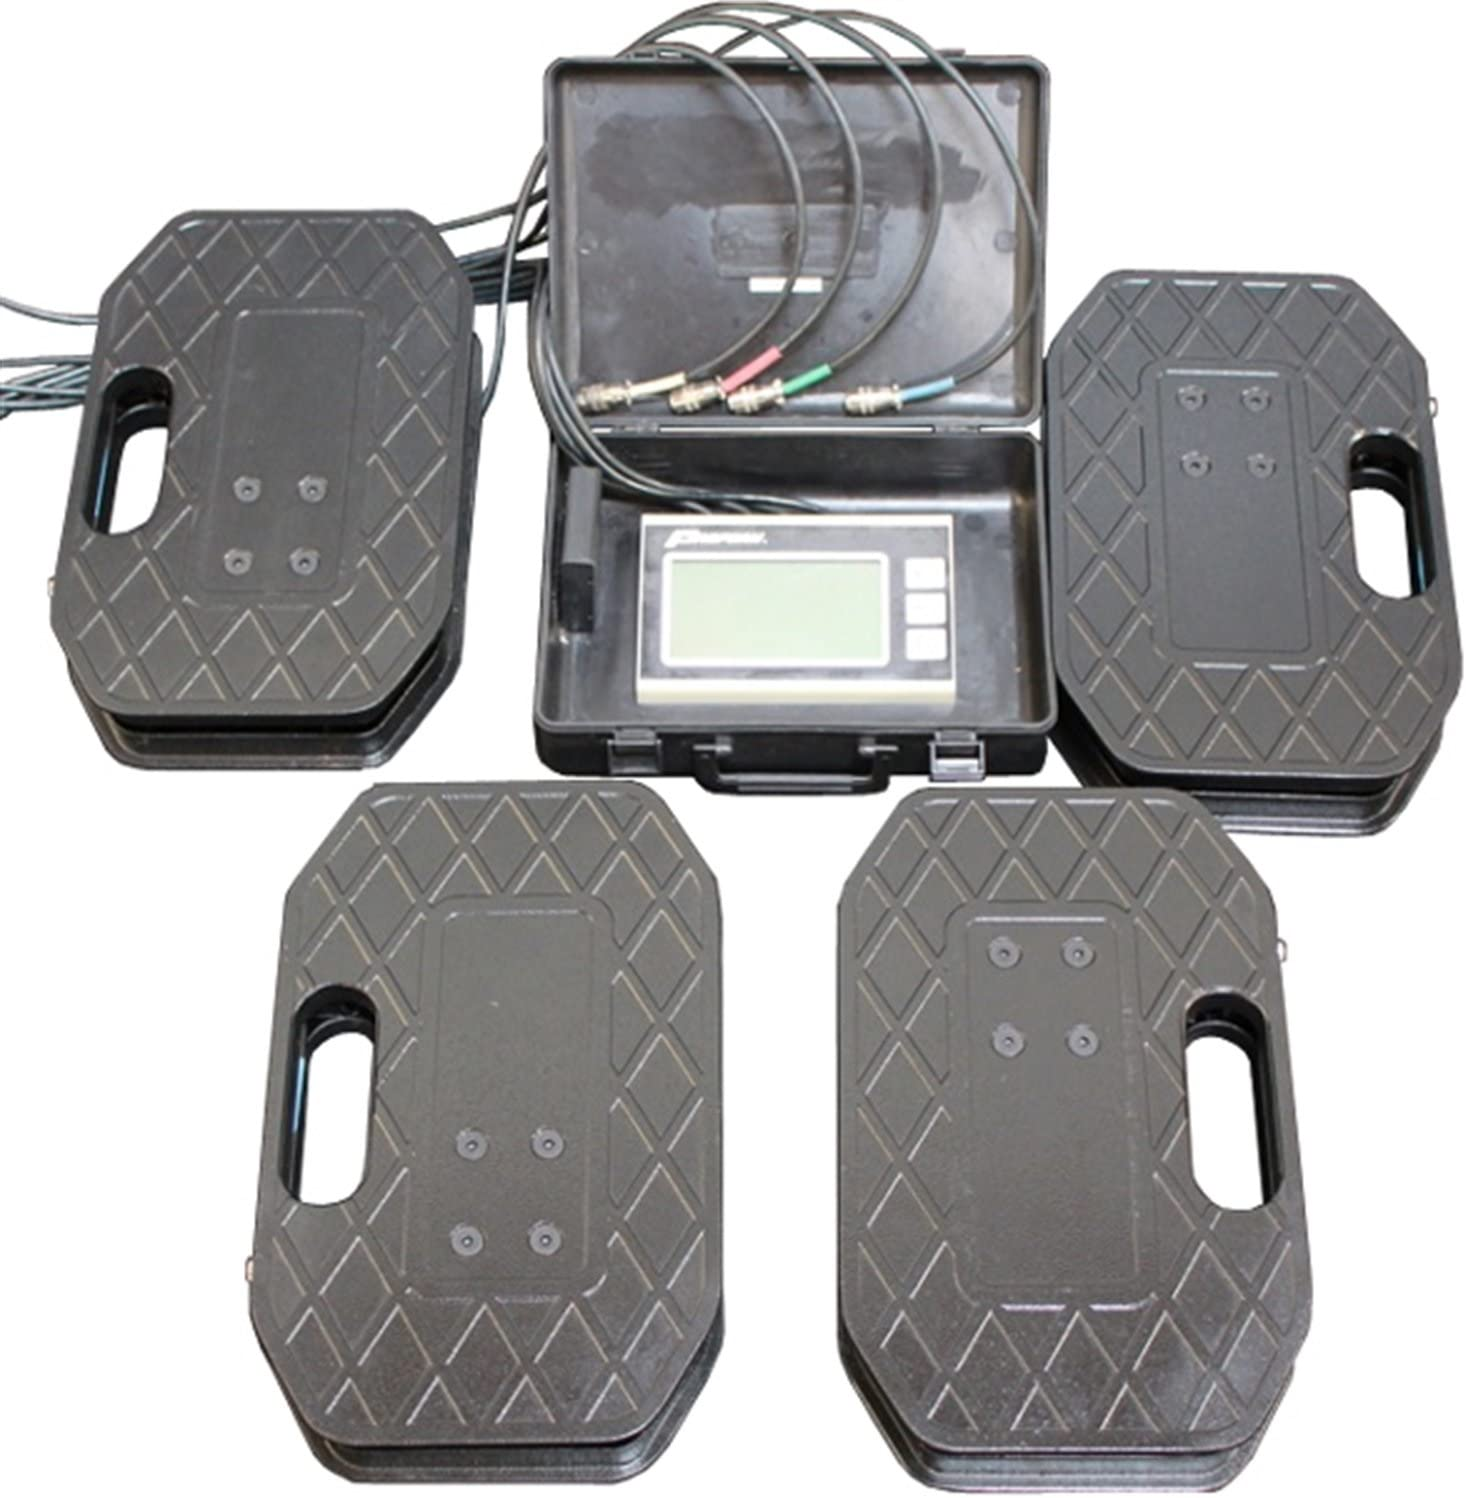
\includegraphics[width=6cm]{
			cornerweithscaleexample}
		\caption{Sistema comercial de Balanças}
		\label{fig:cornerweithscaleexample}
	\end{figure}
	
	\subsection{Inputs}
	A entrada de dados vem dos chips que fazem a leitura das balanças, o HX711. Esses chips funcionam através de um protocolo I2C. Como seria necessário usar 4 chips, um para cada balança, seriam criadas 4 linha de dados I2C, com linha de clock simultâneo. Talvez seja desenvolvida uma eletrônica específica com amplificador operacional para leitura em portas analógicas. Além disso, o Arduíno deve responder a comandos do Usuário para zerar o sistema, alterar unidades e calibrar as balanças; comandos estes que podem ser feitos por um botão individual.
	
	
	\subsection{Outputs}
	A Saída de dados se da pela comunicação com um display LCD 16x2 ou 16x4 que informa ao usuário o peso das balanças e outras informações como distribuição lateral e longitudinal de massa e o peso total do veículo. 
	
	
	\subsection{Processamento e Armazenamento}
	Processamento e aramazenamento de dados ocorre pra ler o dado do chip e efetuar a conversão do dado bruto em um peso em uma determinada unidade. Além disso, as balanças precisam ser calibradas com um peso de calibração (5kg) e com isso se obtêm um dado de calibração que é armazenado na \textit{EEPROM} do \textit{ATMEGA328P} para ser utilizado em todas as medições futuras das balanças. 
	
	\section{Lista de materiais}
	Os materiais usados para a realização do projeto serão totalmente virtuais, o sistema será projetado somente em ambiente de simulação, podendo ser configurado o peso de cada balança pela simulação, assim como demonstrado a operação do display. O software será desenvolvido na Arduino IDE com o FreeRTOS para Arduíno que está disponível neste link \url{https://github.com/feilipu/Arduino_FreeRTOS_Library}.
	
	\subsection{Github}
	O Projeto será hospedado no Github e será usado as ferramentas de colaboração com repositório público acessível pelo link: \url{https://github.com/Eugenio-Pozzobon/Sistema-de-Balancas-Automotivo}
	
	\section{Cronograma}
	\begin{table}[htb]
		\centering
		\begin{tabular}{c|c}
			Atividade & Deadline \\ \hline
			Elaboração do projeto & 05/08/21 \\ \hline
			Envio do plano de projeto & 12/08/21 \\ \hline
			Início do código base do projeto e testes & 14/08/21 \\ \hline
			Finalização do código e testes finais & 19/08/21 \\ \hline
			Preparação da apresentação & 22/08/21 \\ \hline
			Entrega	& 26/08/21\\
		\end{tabular}
	\end{table}
	
	
\end{document}
